\section{Controller software}\label{sec:controllerSoftware}

This section contains documentation of the controller software. The controller software contains the \texttt{manuel} function to control the crane manually, but has also been prepared for automated control with the \texttt{automated} function. It is possible to switch between the two functions using the switch built into the remote, where an LED is implemented to inform the user which function is selected. An LED is also used to indicate whether the switch to toggle the magnet has been press, and also to indicate whether the controller is being powered. The code for the controller is found via the following github link \url{linktilgit}

\subsection{Joystick data conversion}

As the joystick outputs two integers between 0 and 1023 for the x- and y-position, and the motor drivers for the x- and y-motor takes two PWM-signals with a duty cycle between \SI{10}{\%} and \SI{90}{\%} as inputs, a conversion is necessary. The Arduino has a function for generating PWM-signals named \texttt{analogWrite} which converts an integer between 0 and 255 to a \SI{5}{V} PWM-signal with a duty cycle between \SI{0}{\%} and \SI{100}{\%}. In order to linearly increase the PWM-signals from \SI{10}{\%} to \SI{90}{\%} using the \texttt{analogWrite} function, the linear function shown in equation \ref{eq:sec:systemDesign:linearPWM} is used.

\begin{equation}
    f(j_\text{val}) = 0.198 \cdot j_\text{val} + 26
    \label{eq:sec:systemDesign:linearPWM}
\end{equation}

\begin{table}[H]
    \begin{tabular}{l|l l l}
        $j_\text{val}$ & Value for the x- or y-position of the joystick & [-] \\
        \end{tabular}
\end{table}

\subsection{Deadzone calculator}

Two enable pins are used to turn off the x and y motor drivers, when the joystick is in the middle position. The joystick outputs 511 or 512 as x and y value, when being placed in the middle position. Therefore, the x enable pin is set to low when the value x-value of the joystick is between 510 and 513. Likewise, the y enable pin is set to low when the value y-value of the joystick is between 510 and 513.

\subsection{Software endstop}

A software endstop function is employed as a safety feature to ensure that the trolley or head does not exceed the operating area. The software endstop is employed as a function which takes the PWM-signal, minimum position, maximum position and current position as inputs. The functions returns the regulated PWM-signal, and can therefore be used to regulate both the head and the trolley of the crane. 

\begin{comment}
\subsection{Software}

The functionalities described above are implemented as a combined function as shown in figure \ref{fig:sec:systemdesign:manualControllerSoftware}. 

\begin{figure}[H]
    \centering
    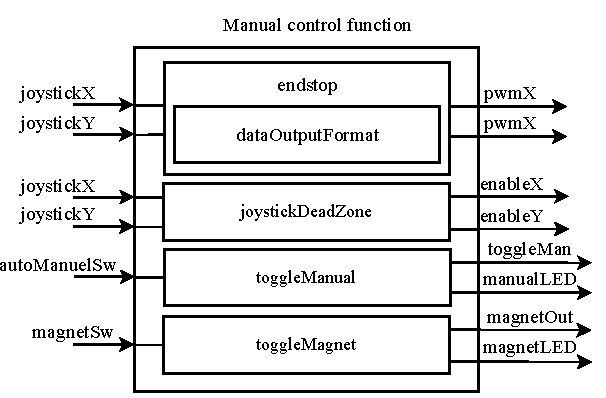
\includegraphics[width = 0.7\textwidth]{pictures/manualControllerFunction (1).pdf}
    \caption{Manual control function.}
    \label{fig:sec:systemdesign:manualControllerSoftware}
\end{figure}

\begin{table}[H]
\centering
\begin{tabular}{|l|l|l|l|}
\hline
\rowcolor[HTML]{C0C0C0} 
Name                 & Functionality                 & Input & Output  \\ \hline
\texttt{endstop}              & Software endstop for x- and y & PWM, min, max, pos & PWM \\ \hline
\texttt{joystickOutputFormat} & Format joystick data          & joystickData & PWM \\ \hline
\texttt{joystickDeadZone}     & Determine deadzone            & joystickData & enableData \\ \hline
\texttt{toggleManual}         & Toggle manual control         & Bool & 0 or 5 V \\ \hline
\texttt{toggleMagnet}         & Toggle magnet                 & Bool & 0 or 5 V \\ \hline
\end{tabular}
\end{table}
\end{comment}